\documentclass[10pt,a4paper]{article}
\usepackage[utf8]{inputenc}
\usepackage[ngerman]{babel}
\usepackage[T1]{fontenc}
\usepackage{amsmath}
\usepackage{amsfonts}
\usepackage{amssymb}
\usepackage{graphicx}
\usepackage{lmodern}
\usepackage{physics}
\usepackage[left=1cm,right=1cm,top=1.5cm,bottom=1.2cm]{geometry}
\usepackage{siunitx}
\usepackage{fancyhdr}
\usepackage{enumerate}
\usepackage{mhchem}
\usepackage{mathtools}
\usepackage{graphicx}
\usepackage{float}
\usepackage{xcolor}
\usepackage{mdframed}
\usepackage{csquotes}
\usepackage{trfsigns}
\usepackage{capt-of}
\usepackage{adjustbox}

\sisetup{locale=DE}
\sisetup{per-mode = symbol-or-fraction}
\sisetup{separate-uncertainty=true}
\DeclareSIUnit\year{a}
\DeclareSIUnit\clight{c}
\mdfdefinestyle{exercise}{
	backgroundcolor=black!10,roundcorner=8pt,hidealllines=true,nobreak
}

\begin{document}
\twocolumn
\pagestyle{fancy}
\lhead{DSV Formelsammlung}
\rhead{Sedlmeier, Toni}
\section{Elementare DSV}
%%%%%%%%%%%%%%%%%%%%%%%%%%%%%%%%%%%%%%%%%%%%% Energie %%%%%%%%%%%%%%%%%%%%%%%%%%%%%%%%%%%%%%%%%%%%%%%%%%%%%
  \subsection{Energie}
  Die Leistung und Energie eines Signals $x(k)$ $k \in [k_1,k_2]$
  \begin{mdframed}[style=exercise]
    \begin{align}
        E_{k_1,k_2} &=\sum_{k=k_1}^{k_2} \abs{x(k)}^2 \ = (k_2 - k_1 +1) P_{k_1,k_2} 
    \end{align}
  \end{mdframed}
  Parsevallsche Gleichung ZDFT:
  \begin{mdframed}[style=exercise]
    \begin{align}
        E_{-\infty,\infty} &=\sum_{-\infty}^{\infty} \abs{x(k)}^2 = \frac{1}{2\pi}\displaystyle\int_{-\pi}^{\pi} \abs{X(e^{j\Omega})}^2 d\Omega
    \end{align}
  \end{mdframed}
  Parsevallsche Gleichung DFT:
  \begin{mdframed}[style=exercise]
    \begin{align}
        E &=\sum_{k=0}^{N-1} \abs{x(k)}^2 =\frac{1}{N}\sum_{n=0}^{N-1} \abs{X(n)}^2 
    \end{align}
  \end{mdframed}
  \subsection{DFT/IDFT}
  \begin{mdframed}[style=exercise]
    \begin{align}
        X(n)&=\sum_{k=0}^{N-1} x(k)e^{-j\frac{2\pi kn}{N}} \\
        x(k)&=\frac{1}{N}\sum_{n=0}^{N-1} X(n)e^{j\frac{2\pi kn}{N}} \\
    \end{align}
  \end{mdframed}
Die DFT bewirkt eine implizite Periodisierung (math. Modulo)
$\tilde{x}(k) = x([k]_{modN})$
  \begin{center}
      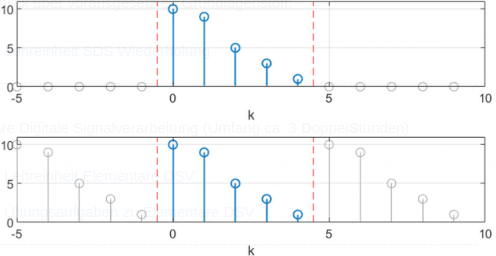
\includegraphics[width=.2\textwidth]{./img/x_k.png}
      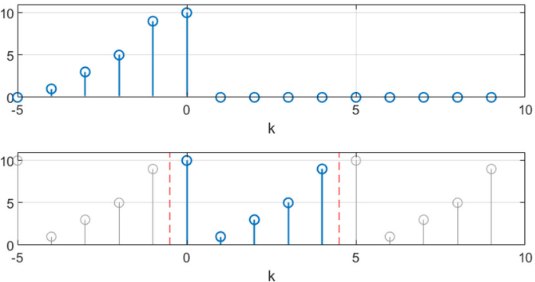
\includegraphics[width=.2\textwidth]{./img/x_mk.png}
  \end{center}
%%%%%%%%%%%%%%%%%%%%%%%%%%%%%%%%%%%%%%%%%%%%%%%%%%%%%%%%%%%%%%%%%%%%%%%%%%%%%%%%%%%%%%%%%%%%%%%%%%%%%%%%%%%%%%%
%%%%%%%%%%%%%%%%%%%%%%%%%%%%%%%%%%%%% DFT-Korrespondenzen %%%%%%%%%%%%%%%%%%%%%%%%%%%%%%%%%%%%%%%%%%%%%%%%%%%%%
\scriptsize
\begin{center}
\begin{tabular}{ | c | c | c | }
\cline{1-3}
        & Zeitbereich & Spektralbereich \\
\cline{1-3}
        Linearität & $a\cdot x_1(k)+ b\cdot x_2(k)$ & $a\cdot X_1(n) +b\cdot X_2(n)$ \\
\cline{1-3}
        Zeit-Verschiebung & $x([k\textcolor{red}{-}k_0]_{modN})$ & $e^{\textcolor{red}{-}j\frac{2\pi nk_0}{N}} X(n)$\\
\cline{1-3}
        Frequenz-Verschiebung & $e^{\textcolor{red}{-}j\frac{2\pi nk_0}{N}} x(k)$ & $X([n\textcolor{red}{+}k_0]_{modN})$ \\  
\cline{1-3}
        Spiegelung & $x([-k]_{modN})$ & $X([-n]_{modN})$ \\  
\cline{1-3}
        Konj.Kompl & $x^*(k)$& $X^*([-n]_{modN})$\\ 
\cline{1-3}
        Konj.Kompl.gespiegelt & $x^*([-k]_{modN})$& $X^*(n)$\\ 
\cline{1-3}
        Faltung & $x_1(k) \circledast x_2(k)$ & $X_1(n)X_2(n)$ \\  
\cline{1-3}
        Multiplikation & $x_1(k)x_2(k)$ & $\frac{1}{N} X_1(n) \circledast X_2(n)$ \\
\cline{1-3}
        gerade Symmetrie & $x_g(k)=\frac{x(k)+\tilde{x}(-k)}{2}$ & $X_g(n)=\frac{X(n)+X(-n)}{2}$ \\
\cline{1-3}
        ungerade Symmetrie & $x_u(k)=\frac{x(k)-\tilde{x}(-k)}{2}$ & $X_u(n)=\frac{X(n)-X(-n)}{2}$ \\
\cline{1-3}
\end{tabular}
\end{center}
% }
%%%%%%%%%%%%%%%%%%%%%%%%%%%%%%%%%%%%%%%%%%%%%%%%%%%%%%%%%%%%%%%%%%%%%%%%%%%%%%%%%%%%%%%%%%%%%%%%%%%%%%%%%%%%
%%%%%%%%%%%%%%%%%%%%%%%%%%%%%%%%%%%%% DFT-Korrespondenzen %%%%%%%%%%%%%%%%%%%%%%%%%%%%%%%%%%%%%%%%%%%%%%%%%%%%%
  \begin{center}
      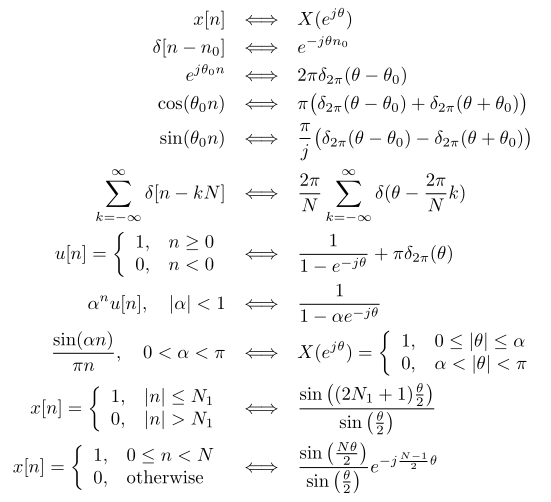
\includegraphics[width=.35\textwidth]{./img/dtft.png}
  \end{center}
  \begin{center}
      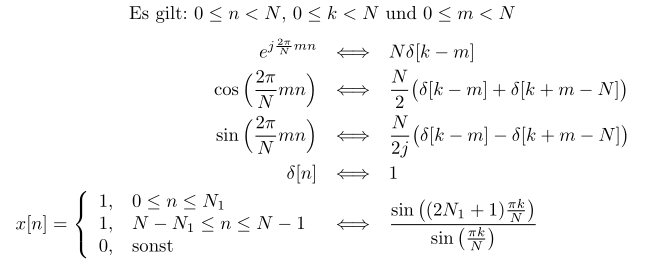
\includegraphics[width=.35\textwidth]{./img/dft.png}
  \end{center}
%%%%%%%%%%%%%%%%%%%%%%%%%%%%%%%%%%%%%%%%%%%%%%%%%%%%%%%%%%%%%%%%%%%%%%%%%%%%%%%%%%%%%%%%%%%%%%%%%%%%%%%%%%%%
%%%%%%%%%%%%%%%%%%%%%%%%%%%%%%%%%%%%% z-Transformation %%%%%%%%%%%%%%%%%%%%%%%%%%%%%%%%%%%%%%%%%%%%%%%%%%%%%
  \subsection{z-Transformation}
  \begin{mdframed}[style=exercise]
    \begin{align}
        X(z) &=\sum_{k=-\infty}^{\infty} x(k)z^{-k} \ \ z=e^{s T_a}
    \end{align}
  \end{mdframed}
%%%%%%%%%%%%%%%%%%%%%%%%%%%%%%%%%%%%%%%%%%%%%%%%%%%%%%%%%%%%%%%%%%%%%%%%%%%%%%%%%%%%%%%%%%%%%%%%%%%%%%%%%%%%
%%%%%%%%%%%%%%%%%%%%%%%%%%%%%%%%%%%%% z-Korrespondenzen %%%%%%%%%%%%%%%%%%%%%%%%%%%%%%%%%%%%%%%%%%%%%%%%%%%%
  \begin{center}
      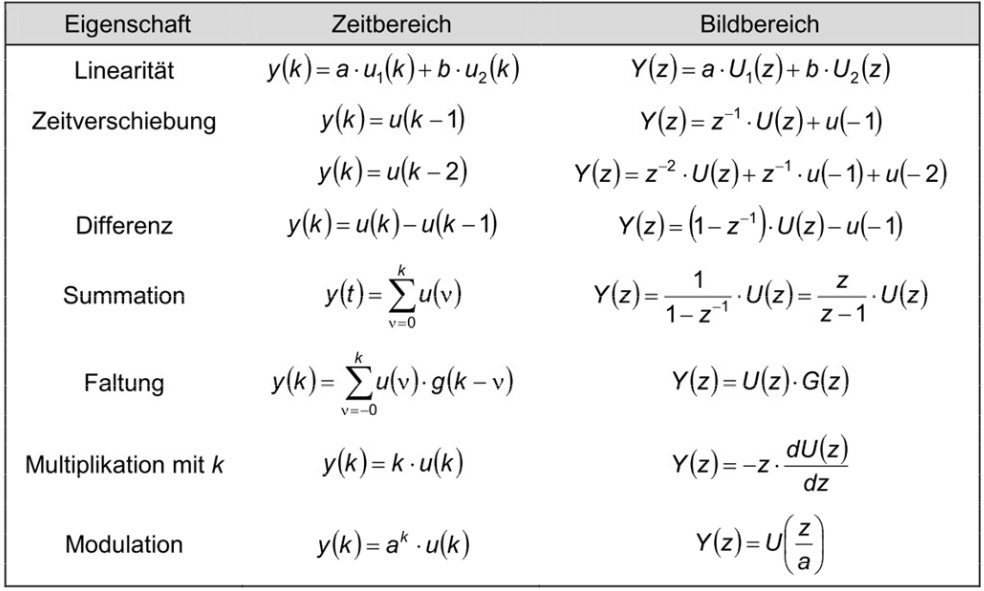
\includegraphics[width=.35\textwidth]{./img/z.png}
  \end{center}
%%%%%%%%%%%%%%%%%%%%%%%%%%%%%%%%%%%%%%%%%%%%%%%%%%%%%%%%%%%%%%%%%%%%%%%%%%%%%%%%%%%%%%%%%%%%%%%%%%%%%%%%%%%%
%%%%%%%%%%%%%%%%%%%%%%%%%%%%%%%%%%%%%%%%%% Faltung %%%%%%%%%%%%%%%%%%%%%%%%%%%%%%%%%%%%%%%%%%%%%%%%%%%%%%%%%
  \subsection{Faltung}
  \subsubsection{Lineare Faltung}
  \begin{mdframed}[style=exercise]
    \begin{align}
        g(k)*u(k) = \sum_{\nu =0}^{k} g(\nu) u(k-\nu)= \sum_{\nu =0}^{k} g(k-\nu) u(\nu)
    \end{align}
  \end{mdframed}
  \subsubsection{Zyklische Faltung}
  $x_1(k)$ und $x_2(k)$ durch \textbf{Zero-Padding} auf $N = N_1 +N_2 -1$ 
  \begin{mdframed}[style=exercise]
    \begin{align}
        x_1(k) \circledast x_2(k) = \sum_{\nu =0}^{N-1} x_1(\nu) x_2([k-\nu]_{modN})= \sum_{\nu =0}^{N-1}x_1([k-\nu]_{modN}) x_2(\nu)
    \end{align}
  \end{mdframed}
%%%%%%%%%%%%%%%%%%%%%%%%%%%%%%%%%%%%%%%%%%%%%%%%%%%%%%%%%%%%%%%%%%%%%%%%%%%%%%%%%%%%%%%%%%%%%%%%%%%%%%%%%%%%
%%%%%%%%%%%%%%%%%%%%%%%%%%%%%%%%%%%%% Korrelation %%%%%%%%%%%%%%%%%%%%%%%%%%%%%%%%%%%%%%%%%%%%%%%%%%%%%%%%%%
  \subsection{Korrelation}
  $x_1(k) \in [0,N_1-1]$ und $x_2(k) \in [0,N_2-1]$
  \begin{mdframed}[style=exercise]
    \begin{align}
        r_{x1x2}(\lambda) = \sum_{k=-\infty}^{\infty}x_1^*(k) x_2(k+\lambda) 
    \end{align}
  \end{mdframed}
%%%%%%%%%%%%%%%%%%%%%%%%%%%%%%%%%%%%%%%%%%%%%%%%%%%%%%%%%%%%%%%%%%%%%%%%%%%%%%%%%%%%%%%%%%%%%%%%%%%%%%%%%%
%%%%%%%%%%%%%%%%%%%%%%%%%%%%%%%%%%%%% Blocksignalverarbeitung %%%%%%%%%%%%%%%%%%%%%%%%%%%%%%%%%%%%%%%%%%%%
  \subsection{Blocksignalverarbeitung}
  Der $i$-te Block $x^{(i)}(k)$ der Länge $L$ mit Versch.abstand $D$ 
  wird als Multiplikation mit Fensterfunktion $w(k)$ beschrieben
  \begin{mdframed}[style=exercise]
    \begin{align}
        Allg.:
        x^{(i)}(k) = x(k+(i-1)D) \cdot w(k)\ \ k\in[0,L-1] 
    \end{align}
  \end{mdframed}
  Überlapp $D_\%$
  \begin{mdframed}[style=exercise]
    \begin{align}
        D_\% = \frac{L-D}{L}100\%
    \end{align}
  \end{mdframed}
% Overlapp-Add
  \subsubsection{Overlapp-Add Verfahren}
  Schnelle Faltung $g(k)*u(k)$ $N_u >> N_g$ 
  Aufteilung $u(k)$ nicht-überlappend (\textbf{nahtlos}) $\rightarrow D=L$ \\
  Zero-Padding $u^{(i)}(k)$ auf $N=L+N_g$ 
% Overlapp-Save
  \subsubsection{Overlapp-Save Verfahren}
  Schnelle Faltung $g(k)*u(k)$ $N_u >> N_g$ \\
  z.B Überlapp = $N_g-1 \rightarrow D=L-N_g+1$ \\
  \begin{mdframed}[style=exercise]
    \begin{align}
        u^{(i)}(k) = u(k+(i-1)D) \ \ k\in[0,L-1]
    \end{align}
  \end{mdframed}
%%%%%%%%%%%%%%%%%%%%%%%%%%%%%%%%%%%%%%%%%%%%%%%%%%%%%%%%%%%%%%%%%%%%%%%%%%%%%%%%%%%%%%%%%%%%%%%%%%%%%%%%%%
%%%%%%%%%%%%%%%%%%%%%%%%%%%%%%%%%%%%% Simultane Transformation %%%%%%%%%%%%%%%%%%%%%%%%%%%%%%%%%%%%%%%%%%%
  \subsection{Simultane Transformation}
  \begin{mdframed}[style=exercise]
    \begin{align}
        x_1(k) = Re[y(k)] = \frac{1}{2}(y(k)+y^*(k))\\
        x_2(k) = Im[y(k)] = \frac{1}{2j}(y(k)-y^*(k))\\
        x_1(k) = x(2k)\\
        x_2(k) = x(2k+1)\\
        y(k) = x_1(k) +jx_2(k)
    \end{align}
  \end{mdframed}
  \begin{mdframed}[style=exercise]
    \begin{align}
        X_1(n) = \frac{1}{2}(Y(n)+Y^*(-n))\\
        X_2(n) = \frac{1}{2j}(Y(n)-Y^*(n))
    \end{align}
  \end{mdframed}

%%%%%%%%%%%%%%%%%%%%%%%%%%%%%%%%%%%%%%%%%%%%%%%%%%%%%%%%%%%%%%%%%%%%%%%%%%%%%%%%%%%%%%%%%%%%%%%%%%%%%%%%%%
%%%%%%%%%%%%%%%%%%%%%%%%%%%%%%%%%%%%% Stochastische Prozesse %%%%%%%%%%%%%%%%%%%%%%%%%%%%%%%%%%%%%%%%%%%
\section{Stochastische Prozesse}
%%%%%%%%%%%%%%%%%%%%%%%%%%%%%%%%%%%%% Stochastische Variable %%%%%%%%%%%%%%%%%%%%%%%%%%%%%%%%%%%%%%%%%%%
\subsection{Wahrscheinlichkeitsdichtefunktion}
Wahrscheinlickkeit $P(x_u \leq x \leq x_o )$, dass $x \in [x_u,x_o]$ 
  \begin{mdframed}[style=exercise]
    \begin{align}
        P(x_u \leq x \leq x_o ) = \displaystyle\int_{x_u}^{x_o} f_x(\alpha) d\alpha \\
        bzw. \ \ F_x(\alpha) = \displaystyle\int_{-\infty}^{\alpha} f_x(u)du\\
        \displaystyle\int_{-\infty}^{\infty} f_x(u)du = 1
    \end{align}
  \end{mdframed}
Gaußverteilung (Normalverteilung)
  \begin{mdframed}[style=exercise]
    \begin{align}
        f_x(\alpha) = \frac{1}{\sigma_x \cdot \sqrt{2\pi}} \cdot e^{-\frac{1}{2} \cdot \left( \frac{\alpha - \mu_x}{\sigma_x}\right)^2}
    \end{align}
  \end{mdframed}
\subsection{Erwartungswert, Varianz}
  \begin{mdframed}[style=exercise]
    \begin{align}
        \mu_x = E[x] = \displaystyle\int_{-\infty}^{\infty} \alpha f_x(\alpha) d\alpha = \displaystyle\sum_{\nu}^{} a_\nu P_\nu\\
        \sigma_x^2 = E[(x-\mu)^2] = E[x]-\mu^2  = \displaystyle\int_{-\infty}^{\infty} (\alpha-\mu_x)^2 \ f_x(\alpha) d\alpha
    \end{align}
  \end{mdframed}
\subsection{Stationärer Stochastischer Prozess}
P. stationär, wenn seine \textcolor{red}{statistischen} Eigenschaften \textcolor{red}{zeitinvariant} sind \\
Einzelner stationärer Stochastischer Prozess:
  \begin{mdframed}[style=exercise]
    \begin{align}
        f_{x(k)}(\alpha) = f_{x(k+k_0)}(\alpha) = f_x(\alpha)
    \end{align}
  \end{mdframed}
Ein Prozess wird zu zwei verschiedene Zeitpunkte $k_1$ und $k_2$
  \begin{mdframed}[style=exercise]
    \begin{align}
        f_{x(k_1)x(k_2)}(\alpha) = f_{x(k_1+k_0)x(k_2+k_0)}(\alpha)
    \end{align}
  \end{mdframed}
Zwei Prozesse $x$ und $y$ wird zu zwei verschiedene Zeitpunkte $k_1$ und $k_2$
\begin{mdframed}[style=exercise]
    \begin{align}
        f_{x(k_1)y(k_2)}(\alpha) = f_{x(k_1+k_0)y(k_2+k_0)}(\alpha)
    \end{align}
  \end{mdframed}
Autokorrelations $\varphi_{xx}(\lambda)$ und Kreuzkorrelation $\varphi_{xy}(\lambda)$
\begin{mdframed}[style=exercise]
    \begin{align}
        \varphi_{xx}(\lambda) = E[x^*(k)x(k+\lambda)] \\
        \varphi_{xy}(\lambda) =E[x^*(k)y(k+\lambda)]
    \end{align}
  \end{mdframed}
Definition \textbf{schwache Stationarität}
\begin{itemize}
    \item $\mu_x = E[x(k)] = const.$
    \item $\varphi_{xx}(\lambda) = \varphi_{xx}(-\lambda)$ (= gerade Symmetrie)
    \item $\varphi_{xx}(0) \geq \abs{\varphi_{xx}(\lambda)}$ (max(Autokorr.) im Ursprung)
    \item $\varphi_{xx}(0) =E[\abs{x(k)}^2]$ (= mittlere Leistung)
    \item $\varphi_{xx}(0) = \sigma_x^2 + \abs{\mu_x}^2$
\end{itemize}
%%%%%%%%%%%%%%%%%%%%%%%%%%%%%%%%%%%%%%%%%%%%%%%%%%%%%%%%%%%%%%%%%%%%%%%%%%%%%%%%%%%%%%%%%%%%%%%%%%%%%%%%%%
%%%%%%%%%%%%%%%%%%%%%%%%%%%%%%%%%%%%% Ergodizität %%%%%%%%%%%%%%%%%%%%%%%%%%%%%%%%%%%%%%%%%%%
\subsection{Ergodizität}
Scharmittelwert und Zeitmittelwert sind aquivalent\\
\scriptsize
\begin{center}
\begin{tabular}{|c|c|c|}
\cline{1-3}
        & Zeitmittelwert(Schätzung) & Scharmittelwert \\
\cline{1-3}
        lin. Mittelwert $\mu_x$ & $\mu_x = \frac{1}{N}\sum_{k=0}^{N-1}x(k)$ & E[x(k)] \\
\cline{1-3}
        Varianz $\sigma_x^2$ & $\sigma_x^2 = \frac{1}{N}\sum_{k=0}^{N-1}\abs{x(k)-\mu_x}^2$ & $E[\abs{x(k)-\mu_x}^2]$ \\
\cline{1-3}
        Autokorr. $\varphi_{xx}(\lambda)$ & $\frac{1}{N}\sum_{k=0}^{N-1} x^*(k)x(k+\lambda) $ & $E[x^*(k)x(k+\lambda)]$ \\
\cline{1-3}
        Kreuzkorr. $\varphi_{xy}(\lambda)$ & $\varphi_{xy}(\lambda)=\frac{1}{N}\sum_{k=0}^{N-1} x^*(k)y(k+\lambda) $ & $E[x^*(k)y(k+\lambda)]$ \\
\cline{1-3}
\end{tabular}
\end{center}
%%%%%%%%%%%%%%%%%%%%%%%%%%%%%%%%%%%%%%%%%%%%%%%%%%%%%%%%%%%%%%%%%%%%%%%%%%%%%%%%%%%%%%%%%%%%%%%%%%%%%%%%%%
%%%%%%%%%%%%%%%%%%%%%%%%%%%%%%%%%%%%% Leistungsdichtespektrum %%%%%%%%%%%%%%%%%%%%%%%%%%%%%%%%%%%%%%%%%%%%
\subsection{Leistungsdichtespektrum LDS}
LDS = DFT der Stochastischen Prozesse \\
Autoleistungsdichtespektrum  $\phi_{xx}(e^{j\Omega})$ und Kreuzeistungsdichtespektrum $\phi_{xy}(e^{j\Omega})$
  \begin{mdframed}[style=exercise]
    \begin{align}
        \phi_{xx}(e^{j\Omega}) = \sum_{\lambda=-\infty}^{\infty} \varphi_{xx}(\lambda) e^{-j\Omega\lambda} \\
        \varphi_{xx}(\lambda) = \frac{1}{2\pi} \displaystyle\int_{-\pi}^{\pi} \phi_{xx}(e^{j\Omega})e^{j\Omega\lambda}d\Omega \\
        \phi_{xy}(e^{j\Omega}) = \sum_{\lambda=-\infty}^{\infty} \varphi_{xy}(\lambda) e^{-j\Omega\lambda} \\
        \varphi_{xy}(\lambda) = \frac{1}{2\pi} \displaystyle\int_{-\pi}^{\pi} \phi_{xy}(e^{j\Omega})e^{j\Omega\lambda}d\Omega
    \end{align}
  \end{mdframed}
Mittlere Leistung $\varphi_{xx}(0)$
  \begin{mdframed}[style=exercise]
    \begin{align}
        \varphi_{xx}(0) = \frac{1}{2\pi} \displaystyle\int_{-\pi}^{\pi} \phi_{xx}(e^{j\Omega})d\Omega  = \frac{\phi_{xx}(e^{j\Omega})}{2\pi}
    \end{align}
  \end{mdframed}
Weißes Rauschen (Mittelwertfrei)
  \begin{mdframed}[style=exercise]
    \begin{align}
        \phi_{xx}(e^{j\Omega}) = \phi_0\\
        \varphi_{xx}(0) = \phi_0 \gamma_0(\lambda)
    \end{align}
  \end{mdframed}
%%%%%%%%%%%%%%%%%%%%%%%%%%%%%%%%%%%%%%%%%%%%%%%%%%%%%%%%%%%%%%%%%%%%%%%%%%%%%%%%%%%%%%%%%%%%%%%%%%%%%%%%%%
%%%%%%%%%%%%%%%%%%%%%%%%%%%%%%%%%%%%% LTI-Systeme %%%%%%%%%%%%%%%%%%%%%%%%%%%%%%%%%%%%%%%%%%%%%%%%%%%%%%%%
\subsection{LTI-Systeme}
  \begin{center}
      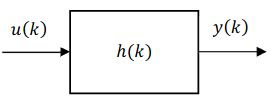
\includegraphics[width=.15\textwidth]{./img/lti.png}
  \end{center}
Mit konst. Mittelwerten $E[u(k-\nu)]=\mu_x$ und $E[y(k)]=\mu_y$
  \begin{mdframed}[style=exercise]
    \begin{align}
        \mu_y = \mu_u \sum_{\nu=-\infty}^{\infty} h(\nu) = \mu_u H(e^{j0})
    \end{align}
  \end{mdframed}
  Zusätzliche Beziehungen
  \begin{mdframed}[style=exercise]
    \begin{align}
        \varphi_{uy}(\lambda) = h(\lambda)*\varphi_{uu}(\lambda) \\
        \varphi_{yu}(\lambda) = h(-\lambda)^**\varphi_{uu}(\lambda) \\
        \varphi_{yy}(\lambda) = h(\lambda)*\varphi_{yu}(\lambda) = h^*(-\lambda)*\varphi_{uy}(\lambda) \\
        \varphi_{yy}(\lambda) = h^*(-\lambda)*h(\lambda)*\varphi_{uu}(\lambda)
    \end{align}
  \end{mdframed}
  \begin{itemize}
      \item $\phi_{uy}(e^{j\Omega}) = H(e^{j\Omega})\phi_{uu}(e^{j\Omega})$
      \item $\phi_{yu}(e^{j\Omega}) = H^*(e^{j\Omega})\phi_{uu}(e^{j\Omega})$
      \item $\phi_{yy}(e^{j\Omega}) = H^*(e^{j\Omega})H(e^{j\Omega})\phi_{uu}(e^{j\Omega}) =\abs{H(e^{j\Omega})}^2 \phi_{uu}(e^{j\Omega}) $ 
  \end{itemize}
%%%%%%%%%%%%%%%%%%%%%%%%%%%%%%%%%%%%%%%%%%%%%%%%%%%%%%%%%%%%%%%%%%%%%%%%%%%%%%%%%%%%%%%%%%%%%%%%%%%%%%%%%%
%%%%%%%%%%%%%%%%%%%%%%%%%%%%%%%%%%%%% Spektralschätzung %%%%%%%%%%%%%%%%%%%%%%%%%%%%%%%%%%%%%%%%%%%%%%%%%%%%%%%%
  \section{Spektralschätzung}
  \subsection{Spektralschätzung mit FFT}
  Umrechnung $n \leftrightarrow f$
  \begin{mdframed}[style=exercise]
    \begin{align}
        f_n = n\frac{f_A}{N}
    \end{align}
  \end{mdframed}
  Umrechnung $\Omega \leftrightarrow n$
  \begin{mdframed}[style=exercise]
    \begin{align}
        \Omega_n = 2\pi\frac{n}{N} = \omega T_a
    \end{align}
  \end{mdframed}
  Umrechnung $\omega \leftrightarrow n$
  \begin{mdframed}[style=exercise]
    \begin{align}
        \omega_n = 2\pi f_A\frac{n}{N} 
    \end{align}
  \end{mdframed}
    \begin{center}
    \begin{tabular}{c c}
        Spektrum & Zeitbereich \\
        $n=0$ & Konstante $x(0)=\frac{1}{N}X(0)$\\
        $n=\tilde{n}$ & $ x_{\tilde{n}}(k)=\frac{1}{N}( X(\tilde{n})e^{-j\frac{2\pi k\tilde{n}}{N}}+X(N-\tilde{n})e^{-j\frac{2\pi k(N-\tilde{n})}{N}})$\\
        $n=\frac{N}{2}$ & $e^{jk\pi} = (-1)^k$\\
    \end{tabular}
    \end{center}
%%%%%%%%%%%%%%%%%%%%%%%%%%%%%%%%%%%%%%%%%%%%%%%%%%%%%%%%%%%%%%%%%%%%%%%%%%%%%%%%%%%%%%%%%%%%%%%%%%%%%%%%%%
%%%%%%%%%%%%%%%%%%%%%%%%%%%%%%%%%%%%% Leck-Effekt %%%%%%%%%%%%%%%%%%%%%%%%%%%%%%%%%%%%%%%%%%%%%%%%%%%%%%%%
\subsection{Leck-Effekt}
Kein Ganzzahliges Vielfaches fällt in das Beobachtungsfenster $w(k)$.\\
Bsp: Sinus $x(t) = sin(w_0t)\cdot w(t)$ mit $w(t)=rect(\frac{t-T/2}{T})$
  \begin{mdframed}[style=exercise]
$        x_w(k) = x(k)w(k) \laplace \  X_w(n) = X(n)*W(n) \\
        sin(w_0t) \fourier j\pi(\delta_0(w+w_0)-\delta_0(w-w_0))\\
        rect(\frac{t-T/2}{T}) \fourier Tsi(w\frac{T}{2})e^{-jw\frac{T}{2}}\\
        X(jw)=\frac{2}{2\pi}[j\pi(\delta_0(w+w_0)-\delta_0(w+w_0))]*si(w\frac{T}{2})e^{-jw\frac{T}{2}}]\\
        X(jw)=j\frac{T}{2}[si((w+w_0)\frac{T}{2})e^{-j(w+w_0)\frac{T}{2}} - si((w-w_0)\frac{T}{2})e^{-j(w-w_0)\frac{T}{2}}]$
  \end{mdframed}
%%%%%%%%%%%%%%%%%%%%%%%%%%%%%%%%%%%%%%%%%%%%%%%%%%%%%%%%%%%%%%%%%%%%%%%%%%%%%%%%%%%%%%%%%%%%%%%%%%%%%%%%%%
%%%%%%%%%%%%%%%%%%%%%%%%%%%%%%%%%%%%% Fensterfunktionen %%%%%%%%%%%%%%%%%%%%%%%%%%%%%%%%%%%%%%%%%%%%%%%%%%%%%%%%
\subsection{Zeitfenster}
  \begin{center}
      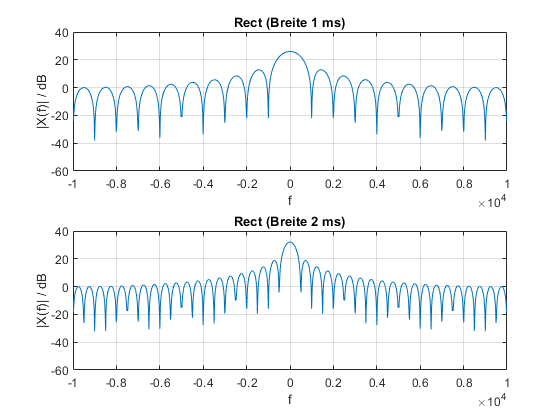
\includegraphics[width=.16\textwidth]{./img/rect.png}
      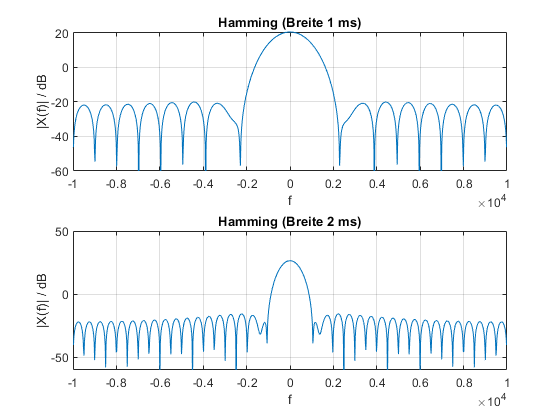
\includegraphics[width=.16\textwidth]{./img/hamming.png}
      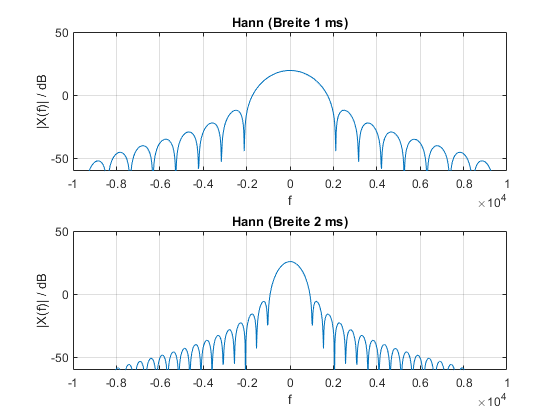
\includegraphics[width=.16\textwidth]{./img/hann.png}
  \end{center}
  Rechteck um bei k=0 beginnend (um $\frac{N}{2}$ verschoben)
  \begin{mdframed}[style=exercise]
    \begin{align}
        rect(k-\frac{N}{2}) \fourier \frac{sin(N\frac{\Omega}{2})}{sin(\frac{\Omega}{2})} e^{-j\Omega\frac{N-1}{2}}
    \end{align}
  \end{mdframed}
\subsection{Zero-Padding}
Zero-Padding = Annäherung an die DTFT $\rightarrow$ feinere Spektrumauflösung Energiegehalt $E = E_{ZP}$ \\
%%%%%%%%%%%%%%%%%%%%%%%%%%%%%%%%%%%%%%%%%%%%%%%%%%%%%%%%%%%%%%%%%%%%%%%%%%%%%%%%%%%%%%%%%%%%%%%%%%%%%%%%%%
%%%%%%%%%%%%%%%%%%%%%%%%%%%%%%%%%%%%% Spektral Stoch. Prozesse %%%%%%%%%%%%%%%%%%%%%%%%%%%%%%%%%%%%%%%%%%%%%%%%%%%%%%%%
\subsection{Spektralschätzung Stoch. Prozesse}
Periodogramm
  \begin{mdframed}[style=exercise]
    \begin{align}
        \hat{\phi}_{Per} = \frac{1}{N}\abs{X(n)}^2
    \end{align}
  \end{mdframed}
Mittlere Leistung P mittels Periodogramm
  \begin{mdframed}[style=exercise]
    \begin{align}
        P = \frac{1}{N}\sum_{n=0}^{N-1} \hat{\phi}_{Per} = \frac{1}{N^2}\sum_{n=0}^{N-1} \abs{X(n)}^2
    \end{align}
  \end{mdframed}
Falls nur Spektrum von $n\in [0,N/2]$ gegeben
  \begin{mdframed}[style=exercise]
    \begin{align}
        P = \frac{1}{N}( \hat{\phi}_{Per}(0) + 2 sum_{n=0}^{N/2-1} \hat{\phi}_{Per} + \hat{\phi}_{Per}(\frac{N}{2})) \\
        P = \frac{1}{N^2}( \abs{X(0)}^2 + 2 \sum_{n=0}^{N/2-1} \abs{X(n)}^2 + \abs{X(N/2)}^2) 
    \end{align}
  \end{mdframed}
Falls nur best. Frequenzintervall $P\in [f_u,f_0] \rightarrow [n_1,n_2]$ 
  \begin{mdframed}[style=exercise]
    \begin{align}
        P = \frac{2}{N}\sum_{n=n_1}^{n_2} \hat{\phi}_{Per} = \frac{2}{N^2}\sum_{n=n_1}^{n_2} \abs{X(n)}^2
    \end{align}
  \end{mdframed}
Auch hier tritt Leck-Effekt auf $\rightarrow$ Minderung mit Fensterfunktion w(t) 
ABER: Verlust von Energie => Modifikation d. Schätzung mit Korrekturfaktor $U$ (hängt von w(t) ab)
Spezialfall: w(t) = rect(t) => U = 1 
  \begin{mdframed}[style=exercise]
    \begin{align}
        \hat{\phi}_{Per,m} = \frac{1}{NU}\abs{X_m(n)}^2\\
        U = \frac{1}{N}\sum_{k=0}^{N-1} \abs{w(t)}^2 
    \end{align}
  \end{mdframed}
%%%%%%%%%%%%%%%%%%%%%%%%%%%%%%%%%%%%%%%%%%%%%%%%%%%%%%%%%%%%%%%%%%%%%%%%%%%%%%%%%%%%%%%%%%%%%%%%%%%%%%%%%%
%%%%%%%%%%%%%%%%%%%%%%%%%%%%%%%%%%%%% Weißes Rauschen %%%%%%%%%%%%%%%%%%%%%%%%%%%%%%%%%%%%%%%%%%%%%%%%%%%%%%%%
\subsubsection{Weißes Rauschen}
LDS ist Konstante $\phi_{xx,WR}(n) = \phi_{xx,WR} = const.$
  \begin{mdframed}[style=exercise]
    \begin{align}
        P = \frac{1}{N} \sum_{n=0}^{N-1} \phi_{xx,WR}(n) = \phi_{xx,WR}
    \end{align}
  \end{mdframed}
%%%%%%%%%%%%%%%%%%%%%%%%%%%%%%%%%%%%%%%%%%%%%%%%%%%%%%%%%%%%%%%%%%%%%%%%%%%%%%%%%%%%%%%%%%%%%%%%%%%%%%%%%%
%%%%%%%%%%%%%%%%%%%%%%%%%%%%%%%%%%%%% Welch-Methode %%%%%%%%%%%%%%%%%%%%%%%%%%%%%%%%%%%%%%%%%%%%%%%%%%%%%%%%
\subsection{Welch-Methode}
Zerlegung von x(k) der Länge N in K Sequenzen $x^{(i)}(k)$ der Länge L. 
Die Startzeitpunkte liegen im Abstand D \\
Es gilt $N=L+D(K-1)$
  \begin{mdframed}[style=exercise]
    \begin{align}
        x^{(i)}(k) = x(k+iD) \ \ k\in[0,L-1] 
    \end{align}
  \end{mdframed}
z.B Fensterung + Zero-Padding $\tilde{L} = L + L_{ZP}$
  \begin{mdframed}[style=exercise]
    \begin{align}
        \hat{\phi}_{Per}^{(i)}(n) = \frac{1}{LU}\abs{X^{(i)}(n)}^2\\
        U = \frac{1}{L}\sum_{k=0}^{N-1} \abs{w(t)}^2 
    \end{align}
  \end{mdframed}
Das LDS ergiebt sich aus \textcolor{red}{Mittelung} aller K Periodogramme
  \begin{mdframed}[style=exercise]
    \begin{align}
        \hat{\phi}_{W}(n) = \frac{1}{K}\sum_{i=0}^{K-1} \hat{\phi}^{(i)}(n) \\
        P = \frac{1}{\tilde{L}}\sum_{n=0}^{\tilde{L}-1}\hat{\phi}_{W}(n)
    \end{align}
  \end{mdframed}
$K\uparrow$ => Varianz d. Schätzung$\downarrow$ => Qualität $\uparrow$\\
$L\downarrow$ => Frequenzauflösung$\downarrow$ \\
$D\downarrow$ => Überlapp$\uparrow$ => K$\uparrow$ => Rechenaufwand$\uparrow$
%%%%%%%%%%%%%%%%%%%%%%%%%%%%%%%%%%%%%%%%%%%%%%%%%%%%%%%%%%%%%%%%%%%%%%%%%%%%%%%%%%%%%%%%%%%%%%%%%%%%%%%%%%
%%%%%%%%%%%%%%%%%%%%%%%%%%%%%%%%%%%%% Digitale-Filter%%%%%%%%%%%%%%%%%%%%%%%%%%%%%%%%%%%%%%%%%%%%%%%%%%%%%%%%
\section{Digitale-Filter}
  \begin{mdframed}[style=exercise]
    \begin{align}
        H(z)=\frac{Y(z)}{U(z)}= \frac{\sum_{\mu=0}^{m} b_\mu z^{-\mu}}{\sum_{\nu=0}^{n} a_\nu z^{-\nu}}
    \end{align}
  \end{mdframed}
Darstellung Linearfaktoren für n=2
  \begin{mdframed}[style=exercise]
    \begin{align}
        H(z)=\frac{b_0(z-z_{01})(z-z_{02})}{a_0(z-z_{\infty 1})(z-z_{\infty 2})}
    \end{align}
  \end{mdframed}
Jeder Linearfaktor kann als von der Frequenz $\Omega$ abhängiger Drehzeiger
\begin{itemize}
    \item Pol verstärkt Amplitudengang
    \item Nullstelle dämpft Amplitudengang
\end{itemize}
\begin{itemize}
    \item $(e^{j\Omega}-z_{01}) = D_{01}e^{j\phi_{01}}$ und $(e^{j\Omega}-z_{02}) = D_{02}e^{j\phi_{02}}$
    \item $(e^{j\Omega}-z_{\infty 1}) = D_{\infty 1}e^{j\phi_{01}}$ und $(e^{j\Omega}-z_{01}) = D_{\infty 2}e^{j\phi_{\infty 2}}$
\end{itemize}
  \begin{center}
      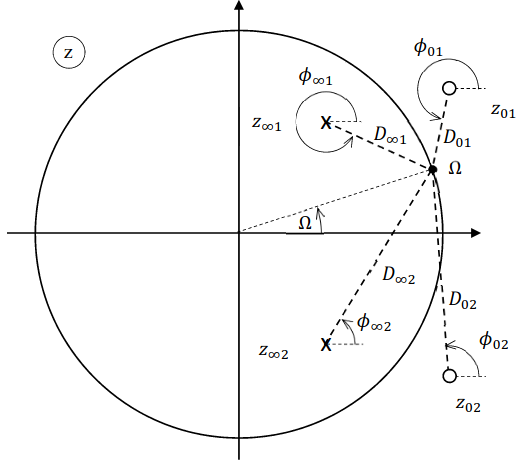
\includegraphics[width=.35\textwidth]{./img/ehk.png}
  \end{center}
\begin{itemize}
    \item Amplitudengang: $\abs{H(e^{j\Omega})}=\abs{\frac{b_0}{a_0}} \abs{ \frac{D_{01}D_{02}}{D_{\infty 1}D_{\infty 2}}}$
    \item Phasengang: $arg({H(e^{j\Omega})})=arg(\frac{b_0}{a_0}) +\phi_{01} +\phi_{02}-\phi_{\infty 1}-\phi_{\infty 2}$
\end{itemize}
%%%%%%%%%%%%%%%%%%%%%%%%%%%%%%%%%%%%%%%%%%%%%%%%%%%%%%%%%%%%%%%%%%%%%%%%%%%%%%%%%%%%%%%%%%%%%%%%%%%%%%%%%%
%%%%%%%%%%%%%%%%%%%%%%%%%%%%%%%%%%%%% Rekursiver Glätter %%%%%%%%%%%%%%%%%%%%%%%%%%%%%%%%%%%%%%%%%%%%%%%%%%%%%%%
\subsection{Rekursiver Glätter}
Vergangenheitswert y(k-1) wird mit Faktor $a\in [0,1]$
  \begin{mdframed}[style=exercise]
    \begin{align}
        y(k) = ay(k-1)+(1-a)u(k) \\
        H(z) =\frac{1-a}{1-az^{-1}}=\frac{(1-a)z}{z-a}
    \end{align}
  \end{mdframed}
Vom Verhalten entspricht er einem Tiefpass 1.Ordnung mit Grenzfrequenz $\Omega_g$ (a lässt sich aus $\Omega_g$ berechnen)
  \begin{mdframed}[style=exercise]
    \begin{align}
        H(e^{j\Omega}) =\frac{1-a}{1-ae^{j\pi\Omega}}\\
        \Omega_g = 2\pi\frac{f_g}{f_A}\\
        a = 2-cos(\Omega_g)-\sqrt{(2-cos(\Omega_g)^2)-1}
    \end{align}
  \end{mdframed}
%%%%%%%%%%%%%%%%%%%%%%%%%%%%%%%%%%%%% Mittelwert %%%%%%%%%%%%%%%%%%%%%%%%%%%%%%%%%%%%%%%%%%%%%%%%%%%%%%%%
\subsection{Arithmetischer Mittelwert Glätter}
  \begin{mdframed}[style=exercise]
    \begin{align}
        y(k)=\frac{1}{N}\sum_{\nu=0}^{N-1} u(k-\nu)\\
        H(z)=\frac{1}{N}\sum_{\nu=0}^{N-1} z^{-\nu} = \frac{1}{N}\frac{z^{-N}-1}{z^{-1}-1}
    \end{align}
  \end{mdframed}
%%%%%%%%%%%%%%%%%%%%%%%%%%%%%%%%%%%%% Notch-Filter %%%%%%%%%%%%%%%%%%%%%%%%%%%%%%%%%%%%%%%%%%%%%%%%%%%%%%%%
\subsection{Notch-Filter}
  \begin{mdframed}[style=exercise]
    \begin{align}
        H(z)=\frac{(z-e^{j\Omega 0})(z-e^{-j\Omega 0})}{(z-r_{\infty}e^{j\Omega 0})(z-r_{\infty}e^{-j\Omega 0})}
    \end{align}
  \end{mdframed}
Vorgabe Kerbe bei Frequenz $f_N$ und -3dB Breite $\Delta f$ und gegebener Abtastfrequenz $f_A$
  \begin{mdframed}[style=exercise]
    \begin{align}
        \Omega_0=\frac{2\pi f_N}{f_A}\\
        \Delta\Omega=\frac{2\pi\Delta f}{f_A}
    \end{align}
  \end{mdframed}
Einsetzen in Übertragungsfunktion H(z) 
  \begin{mdframed}[style=exercise]
    \begin{align}
        H(z)=b\frac{1-2cos(\Omega_0)z^{-1}+z^{-2}}{1-2bcos(\Omega_0)z^{-1}+(2b-1)z^{-2}}\\
        b=\frac{1}{1+\frac{\sqrt{1-G_B^2}}{G_B}tan(\frac{\Delta\Omega}{2})}
    \end{align}
  \end{mdframed}
%%%%%%%%%%%%%%%%%%%%%%%%%%%%%%%%%%%%% Kammfilter %%%%%%%%%%%%%%%%%%%%%%%%%%%%%%%%%%%%%%%%%%%%%%%%%%%%%%%%
\subsection{Kammfilter}
Zu jeder Nullstelle $z_{0n}$ einen Pol $z_{\infty n}$ im Radius $r_\infty<1$ plazieren. p = Ordnung
  \begin{mdframed}[style=exercise]
    \begin{align}
        z_{\infty n} = r_\infty e^{j\frac{2\pi n}{p}} = r_\infty z_{0n} \ \ n\in[0,p-1]
    \end{align}
  \end{mdframed}
Dimensionierung b, sodass zwischen Kerben 0dB(=1)
  \begin{mdframed}[style=exercise]
    \begin{align}
        H(z)=b\frac{1-z^{-p}}{1-r_\infty z^{-p}}\\
        \abs{b\frac{2}{1+r_\infty^p}}\stackrel{!}{=}1 \leftrightarrow b=\frac{1+r_\infty ^p}{2}
    \end{align}
  \end{mdframed}
%%%%%%%%%%%%%%%%%%%%%%%%%%%%%%%%%%%%% Goertzel-Algorithmus %%%%%%%%%%%%%%%%%%%%%%%%%%%%%%%%%%%%%%%%%%%%%%%%%%%%%%%%
\subsection{Goertzel-Algorithmus}
Bestimmung eines einzelnen DFT-Spektralwert X(n). Gleicher Rechenaufwand wie FFT aber Blocklänge N muss keine 2er Potenz sein. $\tilde{x}(k)=[x(0..N-1) \ 0]$ (N-ter Wert 0 setzen)
  \begin{mdframed}[style=exercise]
    \begin{align}
        n_0 = \frac{f_0}{f_A}N\\
        X(n_0)= y(k)=x(k)*h(k)|_{k=N}\\
        X(n_0)=y_n(k)=\sum_{\nu=0}^{k}\tilde{x}(\nu)e^{j\frac{2\pi}{N}(k-\nu)n}
    \end{align}
  \end{mdframed}
%%%%%%%%%%%%%%%%%%%%%%%%%%%%%%%%%%%%% IIR-Filter %%%%%%%%%%%%%%%%%%%%%%%%%%%%%%%%%%%%%%%%%%%%%%%%%%%%%%%%
\subsection{IIR-Filter}
  \begin{mdframed}[style=exercise]
    \begin{align}
        H(z)=\frac{Y(z)}{U(z)}= \frac{\sum_{\mu=0}^{m} b_\mu z^{-\mu}}{\sum_{\nu=0}^{n} a_\nu z^{-\nu}}
    \end{align}
  \end{mdframed}
Gruppenlaufzeit $\tau$ = Verzögerungszeit des Systems aufgelöst nach Frequenzen
  \begin{mdframed}[style=exercise]
    \begin{align}
        \tau = \frac{d}{df}\varphi
    \end{align}
  \end{mdframed}
%%%%%%%%%%%%%%%%%%%%%%%%%%%%%%%%%%%%% FIR-Filter %%%%%%%%%%%%%%%%%%%%%%%%%%%%%%%%%%%%%%%%%%%%%%%%%%%%%%%%
\subsection{FIR-Filter}
grundsätzlich Stabil, Ordnung m $\rightarrow$ m Pole im Ursprung
  \begin{mdframed}[style=exercise]
    \begin{align}
        H(z)=\frac{Y(z)}{U(z)}= \sum_{\mu=0}^{m} b_\mu z^{-\mu} \\
        H(z)=\frac{b_0\Pi_{\mu=1}^{m}(z-z_{0\mu})}{z^m}\\
        h(k)= b_k \ \ k\in[0,m-1] 
    \end{align}
  \end{mdframed}
Gewollte Eigenschaft: \textcolor{red}{lineare Phase}
  \begin{mdframed}[style=exercise]
    \begin{align}
        \tau_g = \frac{d}{d\Omega} arg(H(e^{j\Omega})) = const.
    \end{align}
  \end{mdframed}
lineare Phase wenn Nullstellen von H(z)
\begin{itemize}
    \item auf Einheitskreis
    \item in am Einheitskreis gespiegelten Paaren $z_{01}$ und $\frac{1}{z^*_{01}}$
\end{itemize}
auftreten
  \begin{center}
      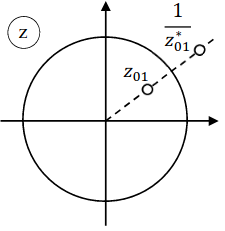
\includegraphics[width=.1\textwidth]{./img/fir.png}
  \end{center}
Für linearphasige FIR-Filter der Ordnung p gilt für Impulsantwort h(k) eine der beiden Symmetrien
\begin{itemize}
    \item $h(k)= h(p-k)$ (gerade Symmetrie) 
    \item $h(k)= -h(p-k)$ (ungerade Symmetrie) 
\end{itemize}

%%%%%%%%%%%%%%%%%%%%%%%%%%%%%%%%%%%%% Kanonische-Formen %%%%%%%%%%%%%%%%%%%%%%%%%%%%%%%%%%%%%%%%%%%%%%%%%%%%%%%%
\subsection{1. Kanonische-Form (IIR)}
Hälfte der Speicherzellen $a_0=1$
  \begin{center}
      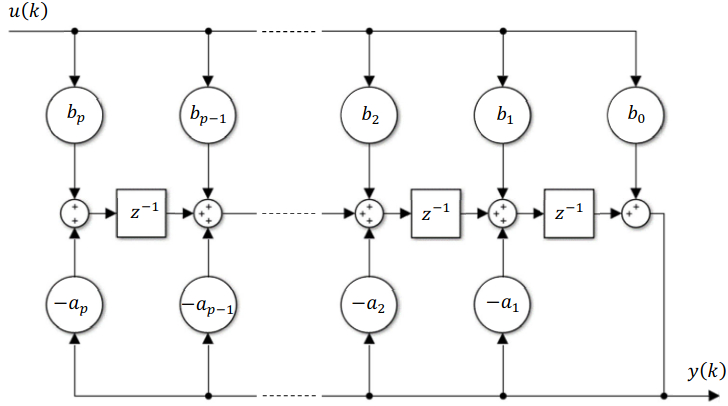
\includegraphics[width=.35\textwidth]{./img/kanon1.png}
  \end{center}
\subsection{2. Kanonische-Form (IIR)}
  \begin{center}
      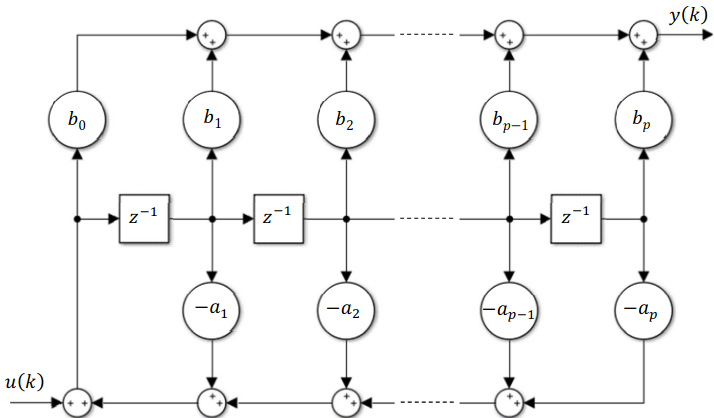
\includegraphics[width=.35\textwidth]{./img/kanon2.png}
  \end{center}
\subsection{3. Kanonische-Form (IIR)}
  \begin{center}
      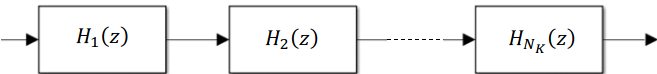
\includegraphics[width=.35\textwidth]{./img/kanon3.png}
  \end{center}
  \begin{mdframed}[style=exercise]
    \begin{align}
        H(z)=\Pi_{\nu=0}^{N_K} H_\nu(z)\\
        H_\nu(z)^{(1)}=\frac{b_{0\nu}+b_{1\nu}z^{-1}}{1+a_{1\nu}z^{-1}}\\
        H_\nu(z)^{(2)}=\frac{b_{0\nu}+b_{1\nu}z^{-1}+b_{2\nu}z^{-2}}{1+a_{1\nu}z^{-1}+a_{2\nu}z^{-2}}
    \end{align}
  \end{mdframed}
\subsection{4. Kanonische-Form (IIR)}
  \begin{center}
      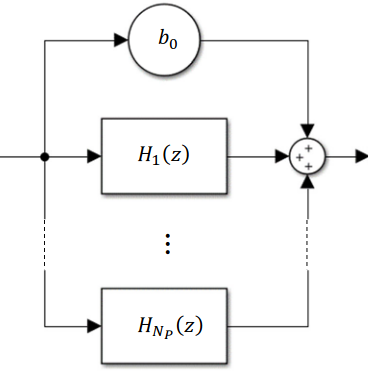
\includegraphics[width=.25\textwidth]{./img/kanon4.png}
  \end{center}
  \begin{mdframed}[style=exercise]
    \begin{align}
        H(z)=b_0+\sum_{\nu=1}^{N_P}H\nu(z)
    \end{align}
  \end{mdframed}
\subsection{Trasversalfilter (FIR)}
Kann effizient durch MAC-Befehl realisiert werden. 
Für linearphasige reelwertige FIR-Filter kann die Symmetrie der $b_k$ genutzt werden.
  \begin{center}
      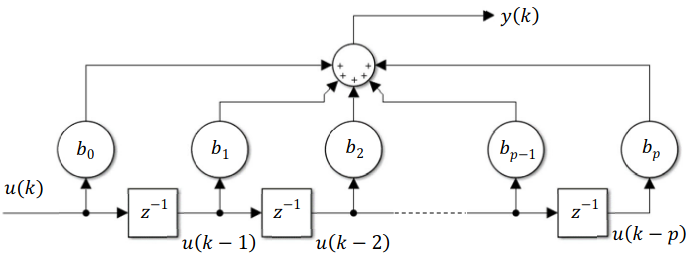
\includegraphics[width=.35\textwidth]{./img/trans.png}
  \end{center}
\subsection{SOS-Faustregel (IIR)}
Aufteilung der Pole-Nullstellen in Biquads, sodass sich Einflüsse auf Frequenzgang ausgleichen.
Vorgehen:
\begin{itemize}
    \item Beginnen mit Pol der am dichtesten am EHK liegt
\end{itemize}
  \begin{center}
      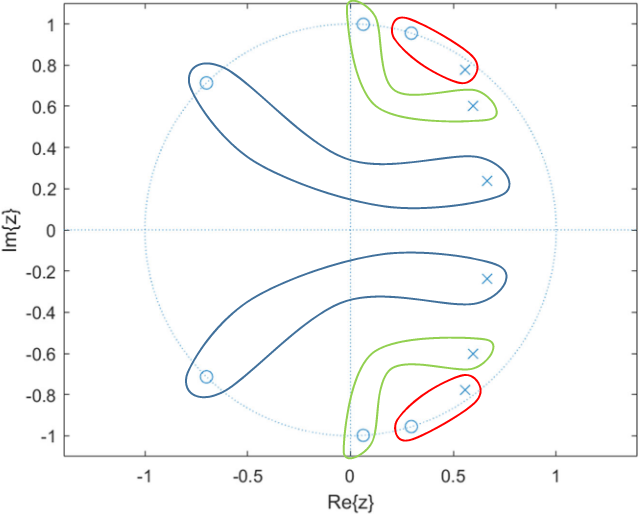
\includegraphics[width=.35\textwidth]{./img/biquad.png}
  \end{center}
%%%%%%%%%%%%%%%%%%%%%%%%%%%%%%%%%%%%%%%%%%%%%%%%%%%%%%%%%%%%%%%%%%%%%%%%%%%%%%%%%%%%%%%%%%%%%%%%%%%%%%%%%%
%%%%%%%%%%%%%%%%%%%%%%%%%%%%%%%%%%%%% Abtastung %%%%%%%%%%%%%%%%%%%%%%%%%%%%%%%%%%%%%%%%%%%%%%%%%%%%%%%
\section{Abtastung}
\subsection{Dezimator Ganzzahliges M}
Dezimator = Kompressor 
  \begin{center}
      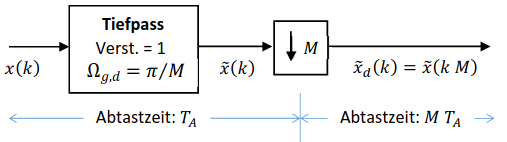
\includegraphics[width=.35\textwidth]{./img/dezi.png}
  \end{center}
Das Spektrum $X(e^{j\tilde{\Omega}})$ des ursprünglichen Signals x(k) wird um $M$ dezimiert,
was zum Spektrum $X_d(e^{j\Omega})$ führt.
  \begin{mdframed}[style=exercise]
    \begin{align}
        x_d(k)=x_c(kMT_A)\\
        X(e^{j\tilde{\Omega}})=\frac{1}{T_A}\sum_{\nu=-\infty}^{\infty} X_c(j\frac{\tilde{\Omega}}{T_A} -\nu\frac{2\pi}{T_A})\\
        X_d(e^{j\Omega})=\frac{1}{MT_A}\sum_{\mu=-\infty}^{\infty} X_c(e^{j\frac{\Omega}{MT_A} -\mu\frac{2\pi}{MT_A}})\\
        % \tilde{\Omega}=\frac{\Omega}{M}-i\frac{2\pi}{M}
        X_d(e^{j\Omega})=\frac{1}{M}\sum_{i=0}^{M-1} X(e^{j\frac{\Omega}{M} -i\frac{2\pi}{M}})\\
    \end{align}
  \end{mdframed}
  \begin{itemize}
    \item Skalierung der Frequenzachse um $\frac{\Omega}{M}$
    \item Verringerung der Periodisierung
    \item Skalierung des Spektrums mit $\frac{1}{M}$
    \item Falls Nyquist-Kriterium $\frac{f_A}{M}>2\tilde{f}_{max}$ nicht erfüllt $\rightarrow$ Hohe Frequenzanteile Tiefpass-Filtern 
  \end{itemize}
  \begin{center}
      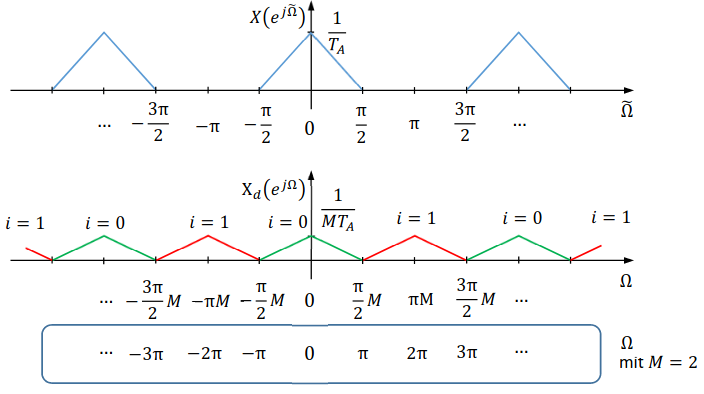
\includegraphics[width=.35\textwidth]{./img/dezi2.png}
  \end{center}
%%%%%%%%%%%%%%%%%%%%%%%%%%%%%%%%%%%%%%%%%%%%%%%%%%%%%%%%%%%%%%%%%%%%%%%%%%%%%%%%%%%%%%%%%%%%%%%%%%%%%%%%%%
%%%%%%%%%%%%%%%%%%%%%%%%%%%%%%%%%%%%% Interpolator %%%%%%%%%%%%%%%%%%%%%%%%%%%%%%%%%%%%%%%%%%%%%%%%%%%%%%%
\subsection{Interpolator Ganzzahliges M}
Interpolator = Expander
  \begin{center}
      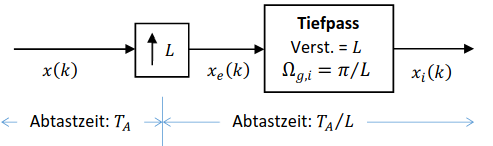
\includegraphics[width=.35\textwidth]{./img/interpol.png}
  \end{center}
Expander hängt hinter jedem Abtastwert von x(k) L-1 0er an.
$x_e(k)= [x(k/L) \ zeros(1,L-1)]$
  \begin{mdframed}[style=exercise]
    \begin{align}
        x_i(k)=x_c(k\frac{T_A}{L})\\
        X_e(e^{j\tilde{\Omega}})=\sum_{\nu=-\infty}^{\infty} x(\nu)e^{-j\Omega\nu L}\\
        X_e(e^{j\Omega}) =X(e^{j\Omega L})
    \end{align}
  \end{mdframed}
  \begin{itemize}
    \item Spektrum $X_e(e^{j\Omega}) =X(e^{j\Omega L})$ läuft von $-\pi/L ...\pi/L$
    \item Keine Skalierung des Spektrums 
  \end{itemize}
  \begin{center}
      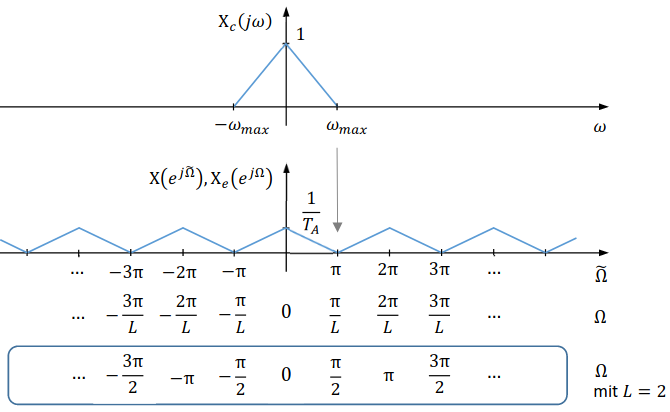
\includegraphics[width=.35\textwidth]{./img/interpol2.png}
  \end{center}
\subsection{Änderung nicht Ganzzahlig}
Zusammenfassung der Tiefpässe zu einem mit V=L und Grenzfrequenz $\Omega_{g,i\&d}=min(\frac{\pi}{L}, \frac{\pi}{M})$
  \begin{mdframed}[style=exercise]
    \begin{align}
        \Omega_{nachher}=\Omega_{vorher}\frac{M}{L}
    \end{align}
  \end{mdframed}
\end{document}
